
\chapter{Metodologia}

{\color{red}Este capítulo dedica-se a prover uma visão geral das etapas necessárias à conclusão deste projeto, e também
permite sua eventual reprodução no futuro.}

Para a execução deste projeto, optou-se pelo uso de componentes amplamente disponíveis no mercado a relativamente baixo
custo, bem como software disponível gratuitamente no site do fabricante.


\section{Hardware}
{\color{red} Esta seção especifica os componentes físicos envolvidos no robô desenvolvido para o projeto, descrevendo
também a função de cada um no desempenho das suas funções.}
{\color{red} Inserir aqui tabela com o custo dos componentes.}

\subsection{Fabricação e montagem}
Foi decido fabricar o chassi e demais peças usando impressão 3D, com PLA.
O projeto das peças foi realizado no AutoCAD e depois modelado em 3D com SolidWorks, após a modelagem realizada,
a geometria das peças foram convertidas em código G para um impressora 3D usando o UltiMaker Cuda, a impressora usada foi a Ender 3 S1 Pro
As figuras relacionadas ao CAD, podem ser encontradas no anexo \ref{att_fabricao_montagem_cad}, quanto a modelagem,
anexo \ref{att_fabricao_montagem_modelagem}, e impressão 3D e montagem, anexo \ref{att_fabricao_montagem_impressao}.



\subsection{Motor DC e driver}
Optou-se pelo uso de um motor DC de 6V 210rpm, com taxa de redução de 1:34. O motor já possui um encoder magnético
acoplado, com 11 PPR (\textit{Pulses Per Revolution}). 
Inicialmente foi testado o driver Ponte H L298N para ligar cada motor, suporta até 2A em operação DC \cite{datasheel_l298n},
a corrente de operação máxima do motor é de 1.1A, porém a corrente de parada é drenar 3.2A. 
O L298N também causa uma queda de tensão, a 1A pode causar uma queda de 3.2V, fazendo com que o
motor não receba a tensão necessária para operar nos valores desejados \cite{datasheel_l298n}. 
O L298N é mais recomendado para tensões entre 12V a 40V, como o motor é de 6v, acaba tendo uma queda de tensão considerável.
Com isso, um driver de para baixas tensões é recomendado, foi escolhido o DRV8833 \cite{datasheel_dvr8833}.

\begin{figure}[h]
	\centering
	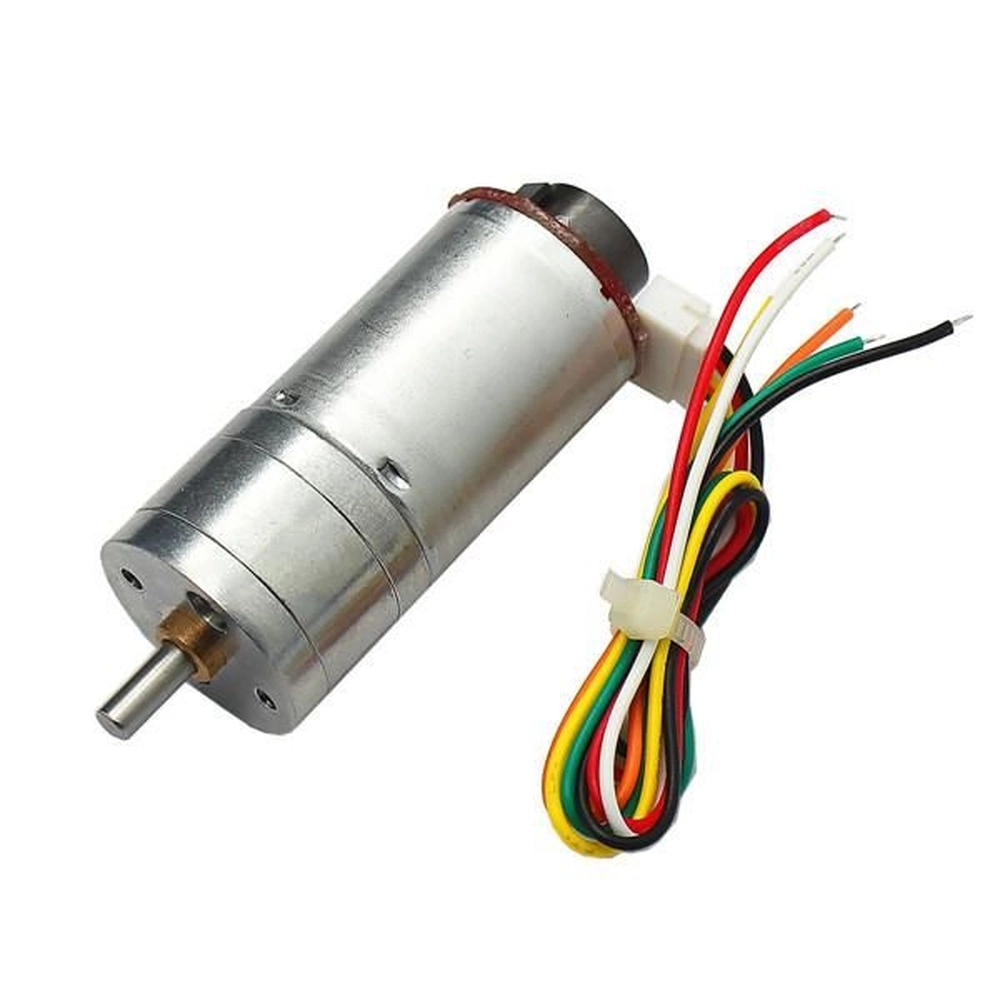
\includegraphics[width=0.7\textwidth]{figures/CHR_GM25_370}
	\caption{Motor DC 6V \cite{motor_dc_6v_encoder}}
\end{figure}


\begin{quadro}[htb]
	\caption{\label{Especificacoes_motordc_6v}Especificações do motor DC 6V}
	 \begin{tabular}{|c|c|c|c|}
		\hline
		\textbf{Componente} & \textbf{Quant} \\ \hline
		Tensão nominal & DC 6V  \\ \hline
		Velocidade sem carga  & 210RPM 0.13A  \\ \hline
		Eficiência máxima & 2,0kg.cm/170rpm/2,0W/0,60A   \\ \hline
		Poder máximo & 5,2kg.cm/110rpm/3,1W/1,10A   \\ \hline
		Torque de parada  & 10kg.cm 3.2A    \\ \hline
		Taxa de Redução do Retardador & 1:34  \\ \hline
		Resolução do salão & Razão Hall x 34,02 = 341,2PPR  \\ \hline
	\end{tabular}
	\fonte{\cite{chinhai_motor}}
	\end{quadro}

\begin{figure}[h]
	\centering
	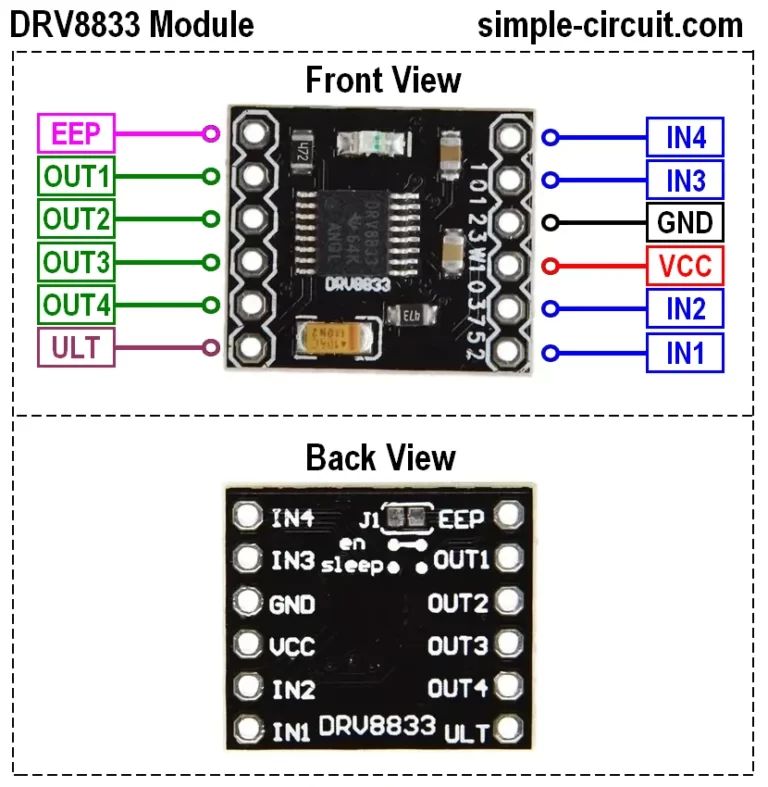
\includegraphics[width=0.7\textwidth]{figures/DRV8833-Dual-Driver-Pinout}
	\caption{Driver Ponte H DVR8833 \cite{DRV8833_image}}
\end{figure}

\subsection{Microcontrolador}

Para microcontrolador, optou-se pelo uso do  STM32F103C8, também conhecido como Blue Pill.
Possui como processador o ARM Cortex-M3, e tem 64Kbs de memória flash. 
O STM32F103C8 possui 7 timers, 2 ADCs, e 9 interfaces de comunicação, incluindo
I2C (\textit{Inter-Integrated Circuit}), USART (\textit{Universal Synchronous
Asynchronous Receiver Transmitter}), SPI (\textit{Serial Peripheral Interface}),
CAN e USB 2.0.
O STM32F103C8 possui 6 que suportam canais de PWM de 5V, e outros 8 canais de 3.3V,  e pode ser alimentado via micro
USB de 5V.

Para carregar o projeto no microcontrolador, um gravador ST-LINK USB será utilizado.

\begin{figure}[h]
	\centering
	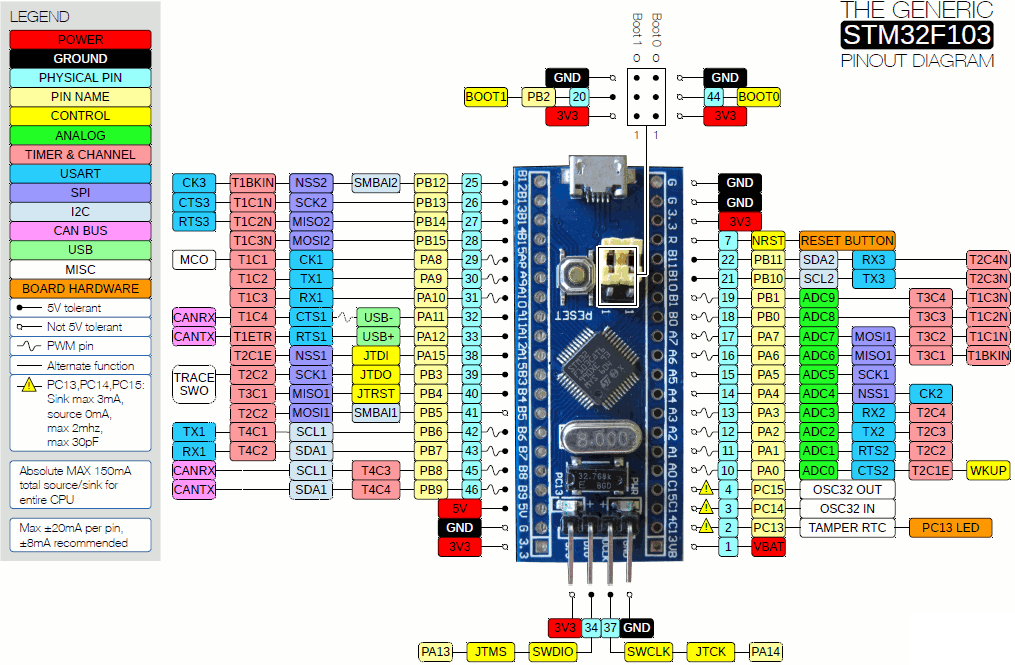
\includegraphics[width=0.8\textwidth]{figures/stm32f1_pinout}
	\caption{Diagrama de pinos do STM32F103C8}
\end{figure}

\subsection{Alimentação}
Para alimentar o microcontrolador, um powerbank com saida de 5v será usado, considerando que o STM32F103C8 funciona a
uma corrente abaixo de 100mA. Para alimentar os motores, para uso no desenvolvimento, optou-se por uma bateria de chumbo-ácido de 6V 4.5Ah

% \subsection{Joystick de controle}
% Um joystick de 3 eixos para controlar o robô para testar a cinemática de movimento.
% {\color{red} É necessário aqui especificar o modelo utilizado e descrever características.}

% \subsection{Sensores}
% {\color{red} Esta subseção deve descrever os sensores utilizados e também sua finalidade.}

% \subsection{Dispositivos de comunicação}
% {\color{red} Esta subseção deve descrever os dispositivos de comunicação utilizados (Wi-fi, Bluetooth, etc) e também sua
% finalidade.}

% \subsection{Calibração de parâmetros}
% {\color{red} Caso haja necessidade de calibração de parâmetros de alguns dos componentes utilizados (sensibilidade de
% sensores, histerese de componentes mecânicos, taxa de comunicação de dispositivos, etc), os procedimentos devem ser
% descritos nesta subseção.}

\section{Software}
{\color{red} Esta seção se dedica a discorrer a respeito dos diversos componentes de software envolvidos no projeto.}

\subsection{Controle de velocidade}

\subsubsection{Medição de velicidade do motor}

Como encoder possuí dois sinais de onda quadadra defasadas em 90º, fase A e fase B, cujos vales e picos são valores lógicos HIGH e LOW, 
e direção de rotação do motor pode ser definida pela diferença entre as fases, se fase A esta adiantada ou atrasada em relação a fase B
É possível calcular a velocidade com base nas subidas da onda quadrada de uma fase, e o valor logico da outra fase no momento da subida.
Por exemplo,  observando a fase B, toda vez em que há uma subida, se o valor da fase A for alto, então incrementar +1 em um contador, se a fase A tiver valor baixo, então incrementar -1 no contador.
Quando o valor da fase A for alto, então o motor esta rodando em um sentido,  quando o valor  for baixo, então o motor esta rodando no sentido contrário.
Medindo o valor do contador por um $\Delta_{T}$, se resulta na quantidade de pulsos por segundo.
Para converter de pulsos por segundo para RPM, basta dividir pela resolução do motor+encoder,  que é de 1:34 do motor, e 11 pulsos por rotação do encoder, o que resulta em 374,
e multiplicar por 60 para ter o resultado em rotações por minuto.

\begin{tikzpicture}[node distance=2cm]

    \node (start) [startstop] {início loop};
    \node (pro1) [process, below of=start] {ENQUANTO DELTA T};
    
    \node (in1) [io, right of=pro1, xshift= 4cm] {QUANDO FASE B = SUBIDA};
    
    \node (dec1) [decision, below of=in1, yshift=-2cm] {SE FASE A = 1};
    \node (pro1a) [process, below of=dec1, yshift= -2cm] {INCREMENTAR CONTADOR em +1};
    \node (pro1b) [process, right of=dec1, xshift= 3cm] {INCREMENTAR CONTADOR em -1};
    
    
    \node (count) [process, below of=pro1, yshift= -9cm] {CONTADOR DIVIDO POR DELTA T};
    
    \draw [arrow] (start) -- (pro1);
    \draw [arrow] (pro1) -- node[anchor=north] {sim} (in1);
    \draw [arrow] (in1) -- (dec1);
    \draw [arrow] (dec1) -- node[anchor=east] {sim} (pro1a);
    \draw [arrow] (dec1) -- node[anchor=north] {não} (pro1b);
    
    \draw [arrow] (pro1) -- node[anchor=east] {não} (count);

\end{tikzpicture}



Na implementação dessa lógica no STM32, o desafio foi a definição do $\Delta_{T}$,
Se o $\Delta_{T}$ for muito pequeno, o resultados de pulsos por segundo pode tender ao infinito, gerando valores muito altos.
Na figura \ref{fig:medidas_altas} em laranja, esta o resultado do rpm considerando o $\Delta_{T}$ como o tempo entre os ciclos do micrcontrolador.
A outra opção, foi definir um $\Delta_{T}$ fixo, definindo uma frequencia de medição pré definida, e o resultado pode ser visto em azul na figura \ref{fig:medidas_altas}
Essa outra opção de $\Delta_{T}$ resultou em um sinal que tem uma componente em alta frequência com uma amplitude até consideral.
Analisando os dois sinai no dominio da frequêcia \ref{fig:frequencia_medidas_altas}, o espectro em frequência do sinal em laranja possui amplitudes muitos semelhante em todo espectro, mas o espectro do sinal em azul, fica bem claro que em altas frequencias é composto mais por ruidos
e as frequencia médias tem amplitude menor em relação as frequências baixas, o que torna mais fácil aplicar um filtro passa-baixa para reduzir as frenquências médias e altas.

A figura \ref{fig:passa_baixa_teste}, mostra um dos teste de filtro passa baixa, em o sinal em laranja ainda persiste esses valores tentendo ao infinito, devido a ampliture eles se tornam um pouco dificil de serem retirados.
Mas o sinal em azul acaba tendo um resultado melhor depois do filtro, muito semelhando ao sinal em laranja.
Com base nesse resultado, foi decidido seguir com o método em que o $\Delta_{T}$ é definido por uma frequência pré definida.


\begin{figure}[h]
    \centering
    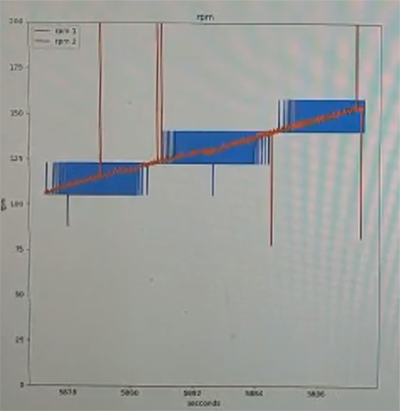
\includegraphics{figures/medidas_altas}
    \caption{Problemas com delta T muito pequeno}
    \label{fig:medidas_altas}
\end{figure}

\begin{figure}[h]
    \centering
    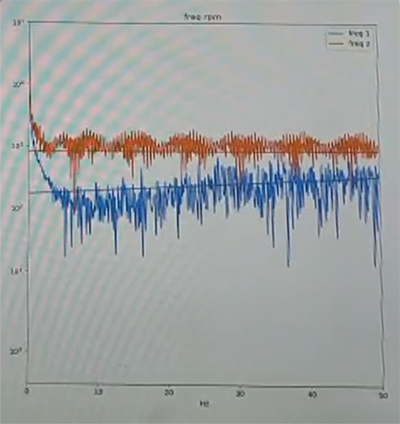
\includegraphics{figures/frequencia_medidas_altas}
    \caption{Frequências}
    \label{fig:frequencia_medidas_altas}
\end{figure}

\begin{figure}[h]
    \centering
    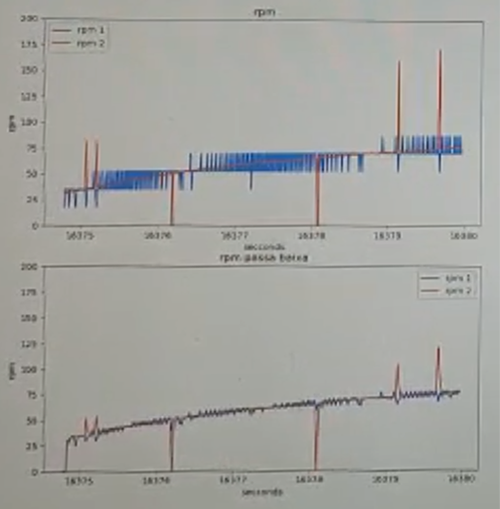
\includegraphics{figures/passa_baixa_teste}
    \caption{Passa baixa teste}
    \label{fig:passa_baixa_teste}
\end{figure}


Com o método definido, foi definido um $\Delta_{T}$ em 100hz eu um filtro passa baixa em 2hz
As imagens no anexo \ref{att_medicao_motores}, mostra as imagens comparando o sinal original e o sinal filtrado para cada motor.
A equação \ref{eqn:equacao_diferenca} a seguir é a equação de diferença do filtro, considerando uma amostragem de 100hz e frequência de corte em 2hz.

\begin{equation}
    \begin{split}
        y[k] = 0.0591174 \cdot u \left[ k \right] +  0.0591174 \cdot u[k - 1] + 0.88176521 \cdot y[k - 1]
    \end{split}
    \label{eqn:equacao_diferenca}
\end{equation}

\subsubsection{Curva PWM x RPM - problema da não linearidade}

Depois de definido como calcular a velocidade o próximo desafio foi lidar com a não linearidade entre o PWM e o resultado medido em RPM.
Como pode ser visto na figura \ref{fig:grafico_pwm_x_rpm}, na comparação entre o valor do PWM e o RPM no tempo.
Considerando essa não linearidade, foram realizadas 15k medições em PWM vs RPM para definir uma equação que pudesse relacionar o PWM com o RPM.
Como pode ser observado na figura  \ref{fig:medicao_pwm_x_rpm_dados_brutos}, os resultados possuem uma tendência, mas possuem alguns pontos fora da curta,
Devido ao esses duídos nas medições ss dados foram tratatos para obter valores médios dos resultados usando python,
o código pode ser visto no anexo \ref{att_limpeza_python}.
O resultado da limpeza dos dados pode ser vizualiado na figura \ref{fig:medicao_pwm_x_rpm_dados_medios}.
Após a limpeza dos dados, os dados foram importados para o matlab, anexo \ref{att_matlab},
para obter um polinômio que possa definir a curva, o polinômio resultante é a equação \ref{eqn:polimonio_rpm}, e a figura \ref{fig:curva_ajustada} representa a curva ajustada.

\begin{equation}
    \begin{split}
        0.0001131x^{4} + -0.03064x^{3} + 2.993x^{2} + -1.257x + 9017
    \end{split}
    \label{eqn:polimonio_rpm}
\end{equation}


\begin{figure}[h]
	\centering
	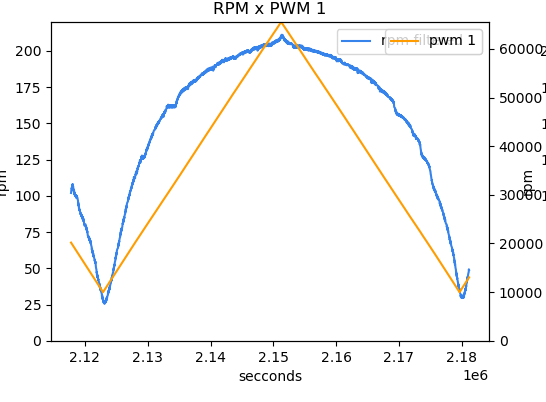
\includegraphics{figures/pwm_x_rpm}
	\caption{Curva PWM e RPM no tempo}
	\label{fig:grafico_pwm_x_rpm}
\end{figure}


\begin{figure}[h]
	\centering
	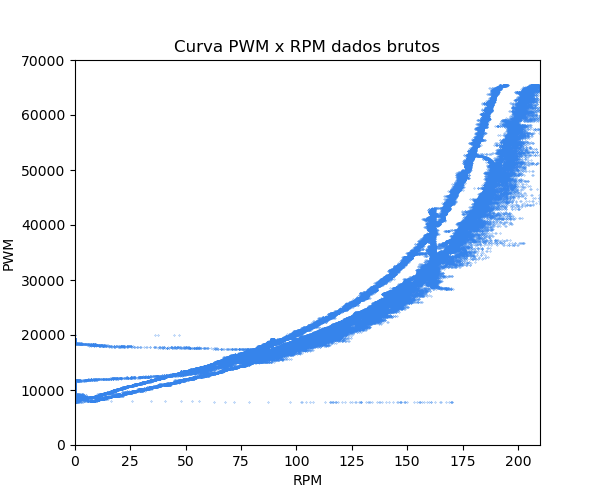
\includegraphics{figures/curva_pwm_x_rpm_dados_brutos}
	\caption{Curva PWM x RPM dados brutos}
	\label{fig:medicao_pwm_x_rpm_dados_brutos}
\end{figure}


\begin{figure}[h]
	\centering
	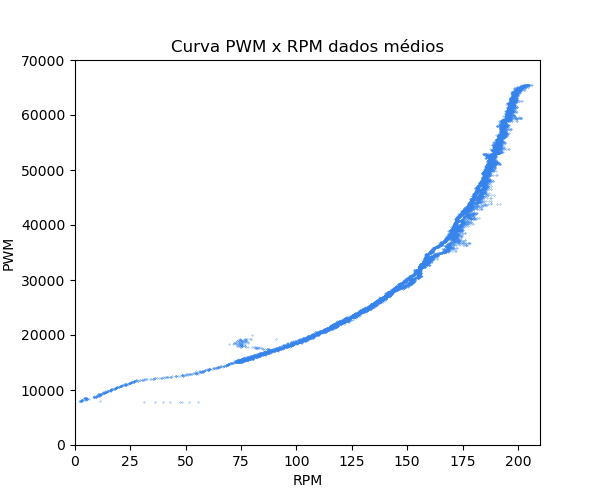
\includegraphics{figures/curva_pwm_x_rpm_dados_medios}
	\caption{Curva PWM x RPM dados médios}
	\label{fig:medicao_pwm_x_rpm_dados_medios}
\end{figure}



\begin{figure}[h]
	\centering
	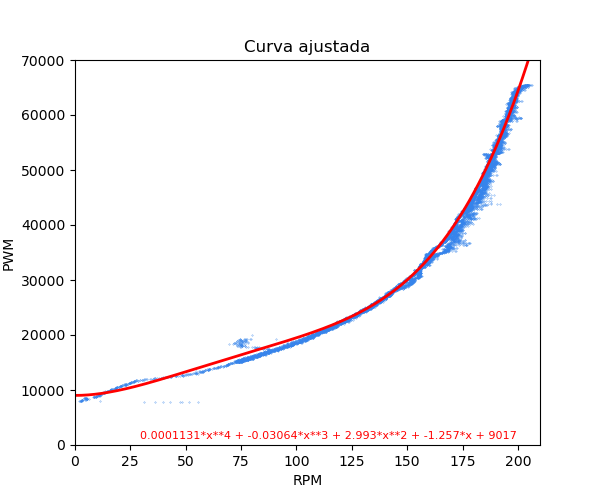
\includegraphics{figures/curva_ajustada}
	\caption{Curva ajustada}
	\label{fig:curva_ajustada}
\end{figure}



\subsection{Controle de posição}
{\color{red} Esta subseção deve descrever como controlar a posição do robô no ambiente interno - presumivelmente, por
meio de sensores e alguma lógica de posicionamento.}

\section{Mapeamento de ambiente}
{\color{red} O objetivo desta seção é descrever a abordagem para mapeamento de ambientes internos - seja carregando um
mapa a partir de coordenadas, ou qualquer outra abordagem adotada.}